\section*{Exercice 188 -- Centre de gravité}
\setcounter{exo}{0}

Soit une portion circulaire de rayon $R$ et de masse linéique $\mu$.

\begin{center}
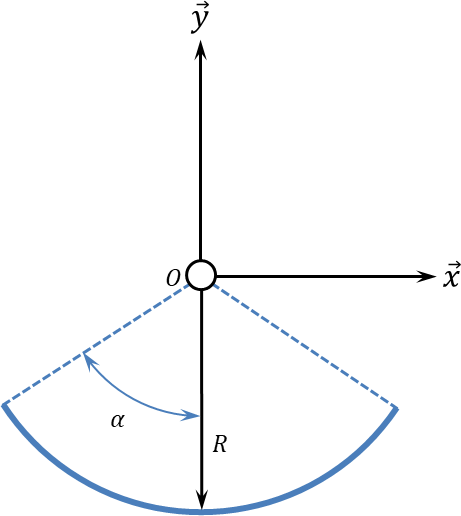
\includegraphics[width=.7\linewidth]{032_01}
\end{center}
\subparagraph{}
\textit{Déterminer les coordonnées du centre d'inertie de cette portion circulaire.}
\ifprof
\begin{corrige}

\end{corrige}
\else
\fi
